\chapter*{{\FontH{\Huge Der Fall der verschwundenen Schmetterlinge}}\\\small \color{red} Papapa gewidmet}
\addcontentsline{toc}{chapter}{Der Fall der verschwundenen Schmetterlinge}



\lettrine[lines=3]{\color{red}D}{as} Mobiltelefon klingelt und weckt Fenja aus dem Schlaf. Es ist noch sehr früh am Morgen, die Sonne ist noch nicht aufgegangen. Es ist noch dunkel und bis auf das Telefon sehr ruhig, wie das um diese Zeit üblich ist. Eine Frechheit, wer ruft denn so früh an? Wäre man nach dem Schlafen doch nicht immer erst so verwirrt. Aha, am Klingelton erkennt Fenja dann doch, dass es Kommissarin Bettina Andermatt sein muss: die Melodie vom rosaroten Panther spielt.

Sofort ist sie hellwach. Fenja geht zwar noch in die Schule, aber sie ist sehr intelligent und kann sehr gut beobachten. Ihr fällt alles auf. Und sie vergisst nie, wann etwas passiert ist, egal wie lang das schon zurück liegt. Ihre Mutter sagt, das hätte sie von Papapa geerbt, als ob immer alles irgendwoher geerbt werden müsste. Aber in dieses Mal hat sie wohl Recht. 

Der Polizei ist es egal, wo ihr Talent genau herkommt, weiss es aber sehr zu schätzen und bittet sie regelmässig, bei der Aufklärung besonders verzwickter Fälle zu helfen. Es scheint wieder einmal soweit zu sein.

\enquote{Ja, aha, ich verstehe.} Fenja schreibt alles, was die Kommissarin sagt, in ein kleines Notizbuch, das immer auf ihrem Nachtschränkchen liegt. Im Papiliorama in Kerzers sind Schmetterlinge verschwunden. Seltene, besonders schöne Exemplare der Gattungen \emph{Morpho peleides}.

\enquote{Entschuldigen Sie die Frage, Frau Kommissarin, aber könnte es sein, dass die Schmetterlinge einfach abgehauen sind? Ich selbst würde auch jede Gelegenheit nutzen, wenn ich so eingesperrt wäre.} Im Zimmer kann man hören, wie die Kommissarin am anderen Ende der Leitung lauter wird. Für vorlaute Spässe habe sie keinen Sinn, schon gar nicht um diese Uhrzeit, hört man sie fast brüllen. Sie erklärt, dass es auffällig ist, dass nur Schmetterlinge eben jener Sorte verschwunden sind. Ausserdem sind auch alle Raupen weg.

Fenja verspricht der Sache sofort am nächsten Morgen nachzugehen und legt auf. Zunächst müssen die organisatorischen Details geklärt werden. Das Papiliorama liegt in Kerzers, das weiss Fenja aber schon. Erst neulich ist sie mit den Grosseltern dort gewesen. Das ist ein schöner Ausflug gewesen. Der erste Zug geht 7:32\,Uhr. Jetzt ist es 4:35\,Uhr. Genügend Zeit, sich vorzubereiten. Folgende Dinge kann Fenja mit Hilfe des Internets bereits recherchieren:

\begin{description}
	\item[Morpho peleides] \sffamily{Deutsch: Blauer Morphofalter. Der Schmetterling gehört zur Familie der Edelfalter. Die Flügel haben blaue Oberseiten und können eine Spannweite bis 12\,cm haben. Sie ernähren sich von faulenden Früchten.}
\end{description}

Fenja staunt. So riesige Schmetterlinge hat sie noch nie gesehen. Mit Hilfe des Lineals macht sie in ihrem Notitzheft ein Quadrat mit einer Höhe und Breite von je zwölf Zentimetern und zeichnet einen Schmetterling. Den malt sie blau aus.

Dann beginnt sie ihren Rucksack zu packen. Sie benötigt:

\begin{enumerate}
  \item Die Detektivausrüstung bestehend aus ein paar sauberen Handschuhen, einer Lupe, einer Pinzette und ein paar leeren kleinen Tüten. Dazu ganz wichtig:0 die gelbe Schnur vom Papapa.
  \item Orangensaft und Käsebrot. Aber ohne Tomaten, nicht wie Papa die belegt, da wird der Käse immer ganz weiss und das findet Fenja ekelig.
  \item Regenjacke, Mütze und Gummistiefel, erfahrungsgemäss finden Verbrecherjagden auch bei Schlechtwetter statt.
  \item Etwas Geld. Damit kann man dann so einiges kaufen, je nachdem, was gebraucht wird. Einmal war es nötig, sofort eine aufblasbare Kuh zu kaufen. Ein sehr merkwürdiger Fall war das damals.
  \item Einen Fotoapparat, um Tatorte dokumentieren zu können. Ein furchtbares Gerät. Es hatte lange gedauert, bis sie gemerkt hatte, dass man beim Bilderbetrachten drücken muss und nicht drehen darf. Grosi hatte es ihr dann gezeigt.
\end{enumerate}

Das alles passt wunderbar in ihren Rucksack. Noch die Schuhe und dann\dots steht plötzlich Carla vor ihr, das ist ihre kleine Schwester. Die wacht immer sehr früh auf und scheint etwas bemerkt zu haben. Carla ist zwar noch ziemlich klein, aber auch nicht dumm. Sofort begreift sie, dass Fenja etwas vor hat. Und sie weiss genau, dass es mit ihrer grossen Schwester immer aufregende Dinge zu erleben gibt.

\enquote{Wenn du mich nicht verrätst, was du planst, fange ich so laut an zu weinen, dass Mama und Papa aufstehen.}

Das hätte gerade noch gefehlt. Die wollen nämlich eigentlich nicht, dass Fenja der Polizei hilft. Viel zu gefährlich meinen sie. Lächerlich. 

\enquote{Was willst du?} fragt Fenja. \enquote{Wenn Du leise bist, erlaube ich Dir so viele Trickfilme auf meinem Computer zu sehen, wie du willst.} Das ist zwar tatsächlich das verführerischste Angebot, dass die grosse Schwester machen kann, aber Carla lässt sich nicht beirren. Fenja seufzt. Ihr bleibt nichts anderes übrig, als Carla alles zu erklären und nach einer kurzen, aber überzeugenden Diskussion auch mitzunehmen. 

\begin{figure}[h]
\centering
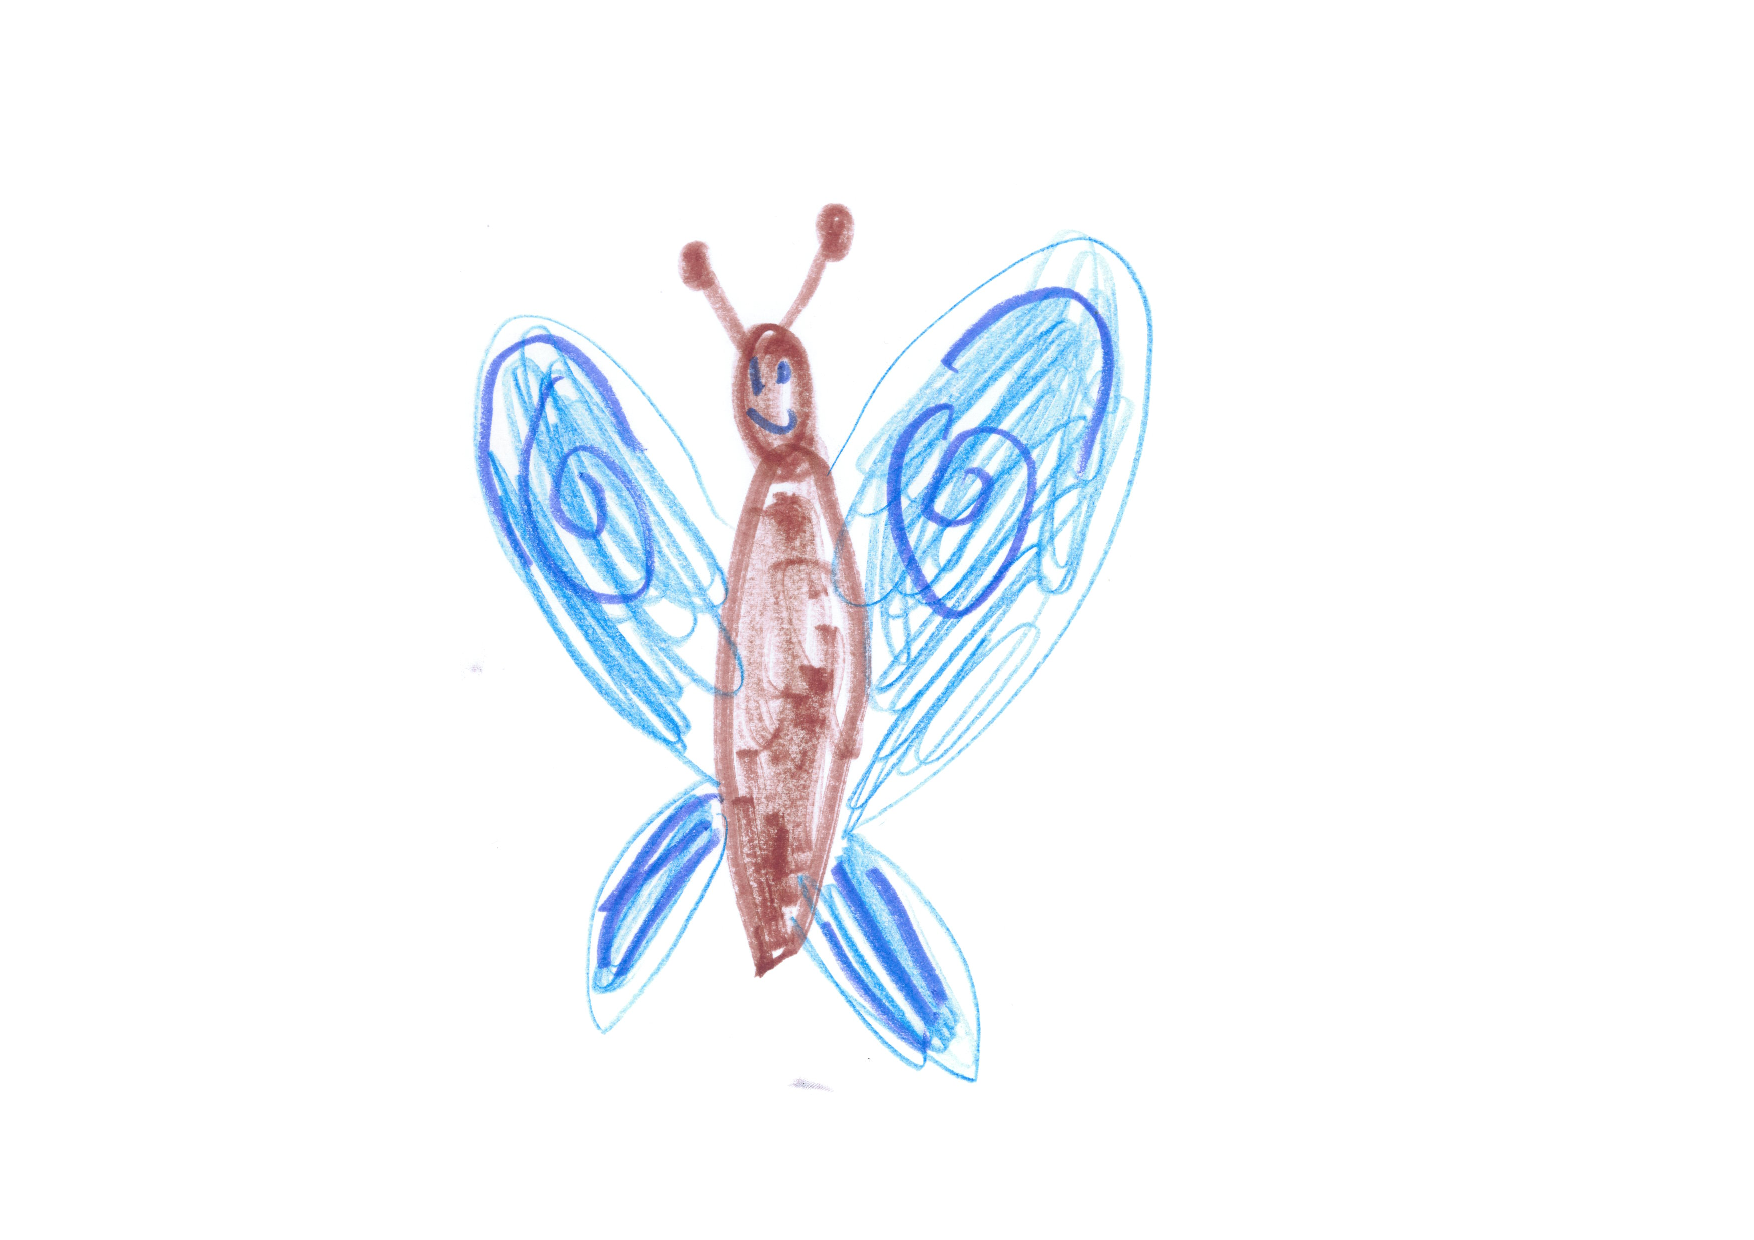
\includegraphics[width=.6\textwidth]{bilder/1blauerSchmetterling.pdf}
\end{figure}
Der Zug erreicht Kerzers pünktlich. Auf dem Weg zum Papiliorama schärft Fenja ihrer Schwester ein, dass sie nicht zum Spass hier sind. Die Schmetterlinge kann man sich auch ein anderes Mal wieder ansehen. Jetzt heisst es ermitteln und Spuren sammeln.

Der Direktor des Papilioramas, Herr Butterblom, weiss, dass Fenja kommen wird. Kommissarin Andermatt hat ihn schon informiert. Fenja entscheidet, dass es das beste ist, sich erst einmal in Ruhe umzusehen, um einen Eindruck vom Tatort zu bekommen. Die beiden Schwestern wollen getrennt ins Papiliorama gehen und sich in einer Stunde in der Cafeteria bei den Süssigkeiten treffen. Niemand wird glauben, dass Carla auch ermittelt.

Fenja hat sich überlegt, dass es sich bei den Dieben der Schmetterlinge nur um Menschen handeln kann, die sich auf irgendeine Art für Schmetterlinge interessieren. Denn wertvoll sind sie nicht.  

\enquote{Herr Butterblom, wer könnte ein Interesse an diesen Schmetterlingen haben?} Fenja weiss, welche Fragen als erstes gestellt werden müssen. Herr Butterblom überlegt.

\enquote{Das weiss ich auch nicht. Es gibt natürlich Leute, die sich für Schmetterlinge interessieren und die selber züchten. Und da kommt es schon einmal vor, dass die hier ein paar Raupen klauen. Aber gleich alle? So etwas ist noch nie passiert.} 

\enquote{Kennen Sie diese Sammler? Können Sie mir vielleicht die Liste aller Namen geben?} will Fenja wissen.

\begin{figure}[H]
\centering
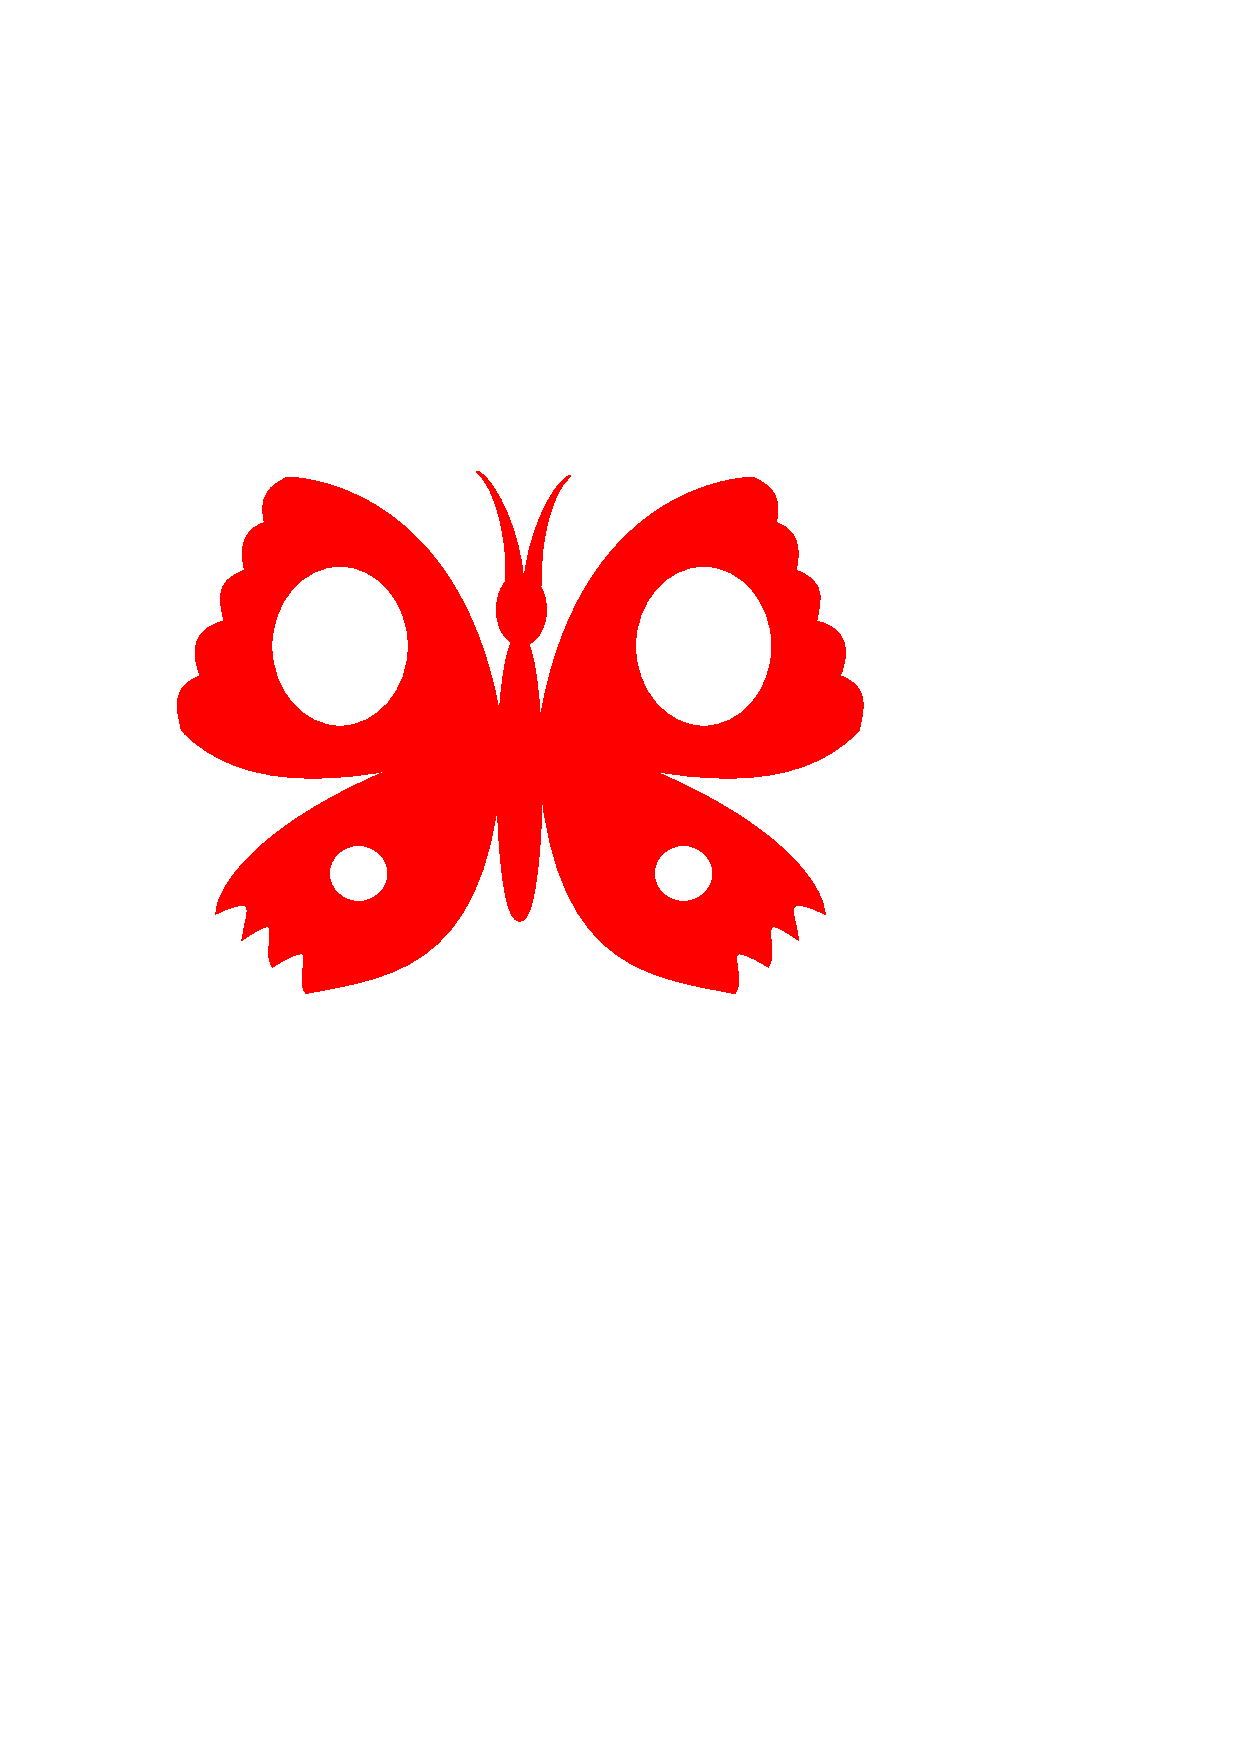
\includegraphics[width=.05\textwidth]{bilder/inkling.pdf}
\end{figure}

\enquote{Natürlich nicht.} antwortet Herr Butterblom. Was für eine Frage. Jetzt kommen ihm doch Zweifel, ob es geschickt von Kommissarin Andermatt war, ein Kind zu schicken. Woher soll er denn die Namen der Leute kennen, die Schmetterlinge züchten? Aber Fenja ist etwas schlauer als er.

\enquote{Auf Ihrer Web-Seite habe ich gesehen, dass Sie auch Tagungen zu Schmetterlingen organisieren. Gerade letzte Woche hat jemand von der Universität einen Vortrag zu Schmetterlingen in den Alpen gehalten.} Fenja ist wirklich sehr gut vorbereitet. 

\enquote{Ich denke, dass alle, die sich für Schmetterlinge interessieren, auch an solchen Veranstaltungen teilnehmen. Es wäre sehr hilfreich, wenn Sie mir die Teilnehmendenliste der letzten beide Jahre per E-Mail schicken könnten.}

Herr Butterblom ist verblüfft. Tatsächlich. Wenn es Züchter gibt, dann kommen die auch hierher und bei Veranstaltungen muss man immer vorher seinen Namen nennen, damit man reservieren kann. 

Nachdem sich Fenja bei Herrn Butterblom bedankt hat, sieht sie sich den Tatort nochmals genau an. Tatsächlich scheint es sehr leicht zu sein, eine unbeobachtete Ecke im Papiliorama zu finden, von der aus man mit einem geeigneten Köder die Schmetterlinge anlocken und dann einfangen kann. Auch der Brutkasten mit den Kokons ist leicht zugänglich. Es ist auch nicht auffällig hier, eine grosse Tasche mit sich zu führen. Es gibt viele Familien und nicht einmal ein richtiges Restaurant. Einige Eltern haben sogar Kühlboxen mit. So komme ich nicht weiter, überlegt Fenja. Es könnte jeder Besucher gewesen sein.
\begin{figure}[H]
\centering
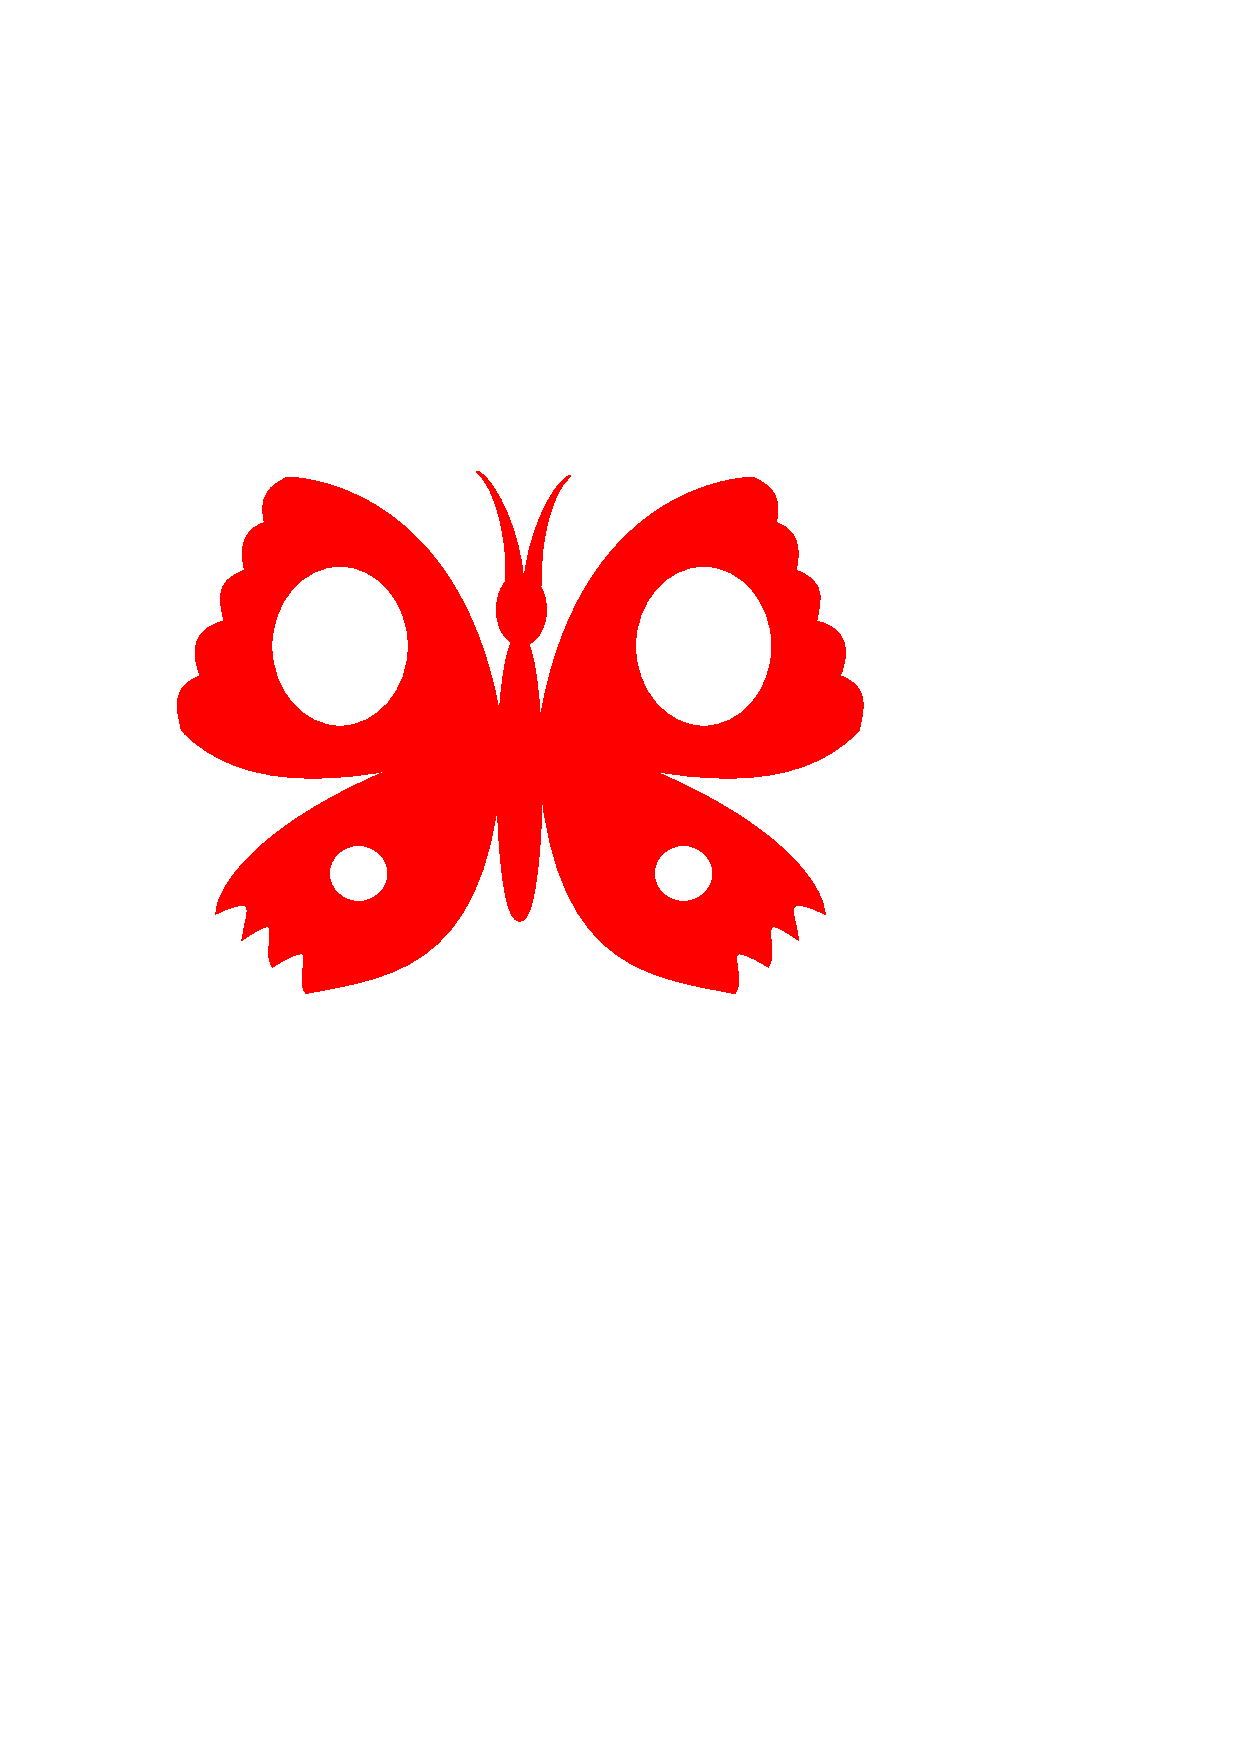
\includegraphics[width=.05\textwidth]{bilder/inkling.pdf}
\end{figure}
Zur selben Zeit schlendert Carla durch die Gänge des Papilioramas. Es läuft gerade eine Sonderausstellung zum Thema \emph{Schmetterlinge in der Kunst}. Künstlerinnen und Künstler aus der Umgebung wurden eingeladen, ihre Sicht auf Schmetterlingen zu zeigen. Jemand hat einen grossen Schmetterling aus Stahl geschweisst, das ist das auffälligste Ausstellungsstück. Daneben gibt es ein paar Bilder an der Wand und eine Designerin hat sogar Kleidungsstücke mit Schmetterlingen bedruckt. Carla fotografiert alles sorgfältig mit der Kamera von Fenja.

\enquote{Alles grosser Unfug! Ganz schreckliches Zeug.} hört Carla neben sich sagen. Eine gross gewachsene Frau mit einem sehr eigenartigen Hut blickt verächtlich auf die ausgestellten Dinge. Carla fragt:

\enquote{Ihnen gefallen die Bilder wohl nicht besonders?}

\enquote{Natürlich nicht.} ruft die Frau mit sich überschlagender Stimme. \enquote{Das ist doch alles Unfug. Neben der Schönheit der Farben eines echten Schmetterlings, ist das hier alles blass und langweilig.} Und dann ergänzt sie:

\enquote{Darf ich mich übrigens vorstellen? Mein Name ist Verena Studer-Matt und der Rock dahinten} dabei deutet sie auf die schmetterlingsgemusterten Kleidungsstücke, \enquote{sind übrigens von mir entworfen. Aber auch die finde ich mittlerweile ganz grauenvoll. Wer einmal die Schönheit eines Blauen Morphos gesehen hat, ist für derartiges verloren.} 


Mit einer Miene, die tiefen Ekel ausdrücken soll und ohne eine Antwort von Carla zu erwarten stapft die Dame davon. Ob sie weiss, dass gerade diese Schmetterlinge alle verschwunden sind, überlegt Carla?

Die beiden Schwestern treffen sich wie verabredet in der Cafeteria. Wie immer darf sich Carla nichts kaufen sondern muss das essen, was Fenja mitgebracht hat. Fenja erzählt kauend, dass man als nächstes bei den Sammlern und Züchtern nachfragen muss. Es sind im Moment die einzigen Verdächtigen. Und weil klar ist, dass sie hier nicht weiterkommen, beschliessen sie nach Bern zu fahren, an der Universität gibt es einen Spezialisten für Schmetterlinge. Das ist der, der neulich hier den Vortrag gehalten hat, am besten man fängt bei dem gleich an. Vielleicht hat der eine Ahnung, wer wohl ein Motiv hat, Schmetterlinge zu stehlen.
\begin{figure}[H]
\centering
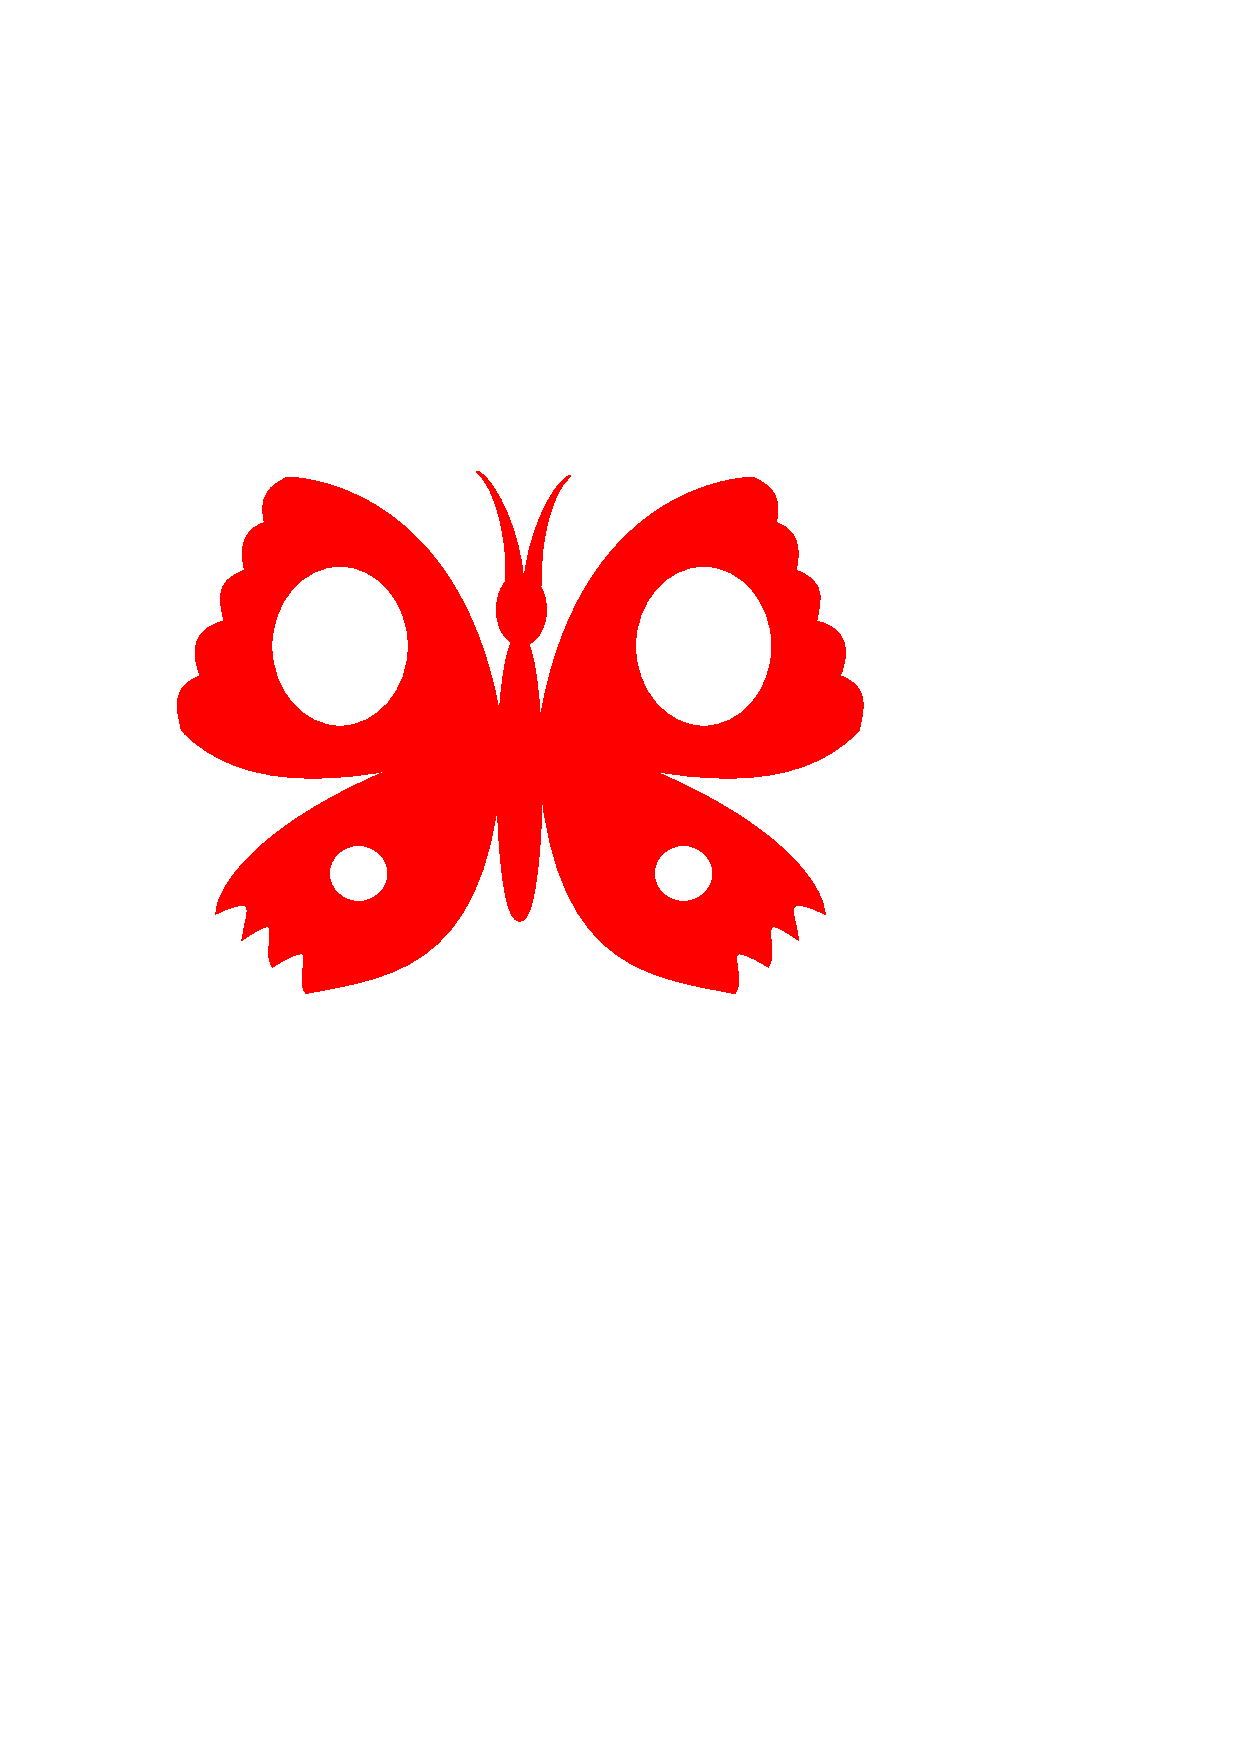
\includegraphics[width=.05\textwidth]{bilder/inkling.pdf}
\end{figure}
Als sie in Bern ankommen, hat Fenja schon über das Internet herausgefunden, wie sie zur Universität kommen und wo sie dort den Schmetterlingsexperten finden, der heisst Dr.\,Adrìan Moreira. \emph{Zoologisches Institut} steht über der Eingangstür. Als ob Fenja jeden Tag hier wäre, geht sie zielsicher zum Fahrstuhl und drückt den Knopf zum dritten Stock. Woher ihre Schwester wohl immer so genau weiss was zu tun ist, überlegt Carla.

\enquote{Hallo ich bin Adrìan} begrüsst sie ein junger Mann mit stark spanischem Akzent. Das verblüfft dann sogar Fenja. Sie hätte sich Professoren viel älter vorgestellt und das sagt sie ihm auch, um sicher zu gehen, dass sie mit dem richtigen spricht. Adrìan muss lachen. \enquote{Na erstens bin ich noch kein Professor und ausserdem seid ihr beiden ja auch nicht im typischen Alter von Detektivinnen.} Er schiebt beiden eine Dose Cola hin. Zu Hause darf Carla die nie trinken, was sie aber jetzt natürlich nicht stört. Nichts anmerken lassen, heisst es jetzt.

\enquote{Also, wie kann ich Euch helfen?} Fenja erklärt was passiert ist. Adrìan hört sehr aufmerksam zu.

\enquote{Nein. Da kann ich euch nicht helfen. Ich habe keine Ahnung, wer so etwas tun könnte. Aber halt, wartet einmal. Neulich war eine Dame hier, die hat sich genau für diesen Schmetterling interessiert. Und die wollte wissen, wie man es am besten schafft, dass die Flügel auch nach dem Tod der Schmetterlinge möglichst lange halten und ihr Blau behalten.}

\enquote{Wie heisst die Frau?} Fenja ist wie elektrisiert. Das ist die erste echte Spur. So etwas kann kein Zufall sein. Adrìan überlegt und schaut in seinem Computer nach.

\enquote{Ich befürchte, dass ich den nicht kenne. Ich glaube, die hat sich gar nie richtig vorgestellt. Aber ich kann sie euch beschreiben. Sie ist schon etwas älter, gross und wenn ihr mich fragt\dots} und statt etwas zu sagen tippt er sich mit dem Finger an die Stirn \enquote{Na jedenfalls hatte sie einen wirklich exzentrischen Hut auf. Riesig und mit Federn.} Jetzt ist Carla aufgeregt. 

\enquote{Die habe ich heute gesehen, im Papliliorama. Das ist die Frau, die die Kleider mit dem Schmetterlingsmuster gemacht hat!} Adrìan und Fenja sehen Carla verblüfft an. Carla erinnert sich, dass die Frau auch ihren Namen genannt hatte, aber den hat sie längst vergessen. Namen kann sie sich einfach nicht merken. Und bevor Fenja böse ist, sagt sie lieber nicht, dass sie den Namen kennen sollte.

\enquote{Wie die heisst, weiss ich auch nicht, aber ich habe die Kleider fotografiert.} Adrìan und Carla blicken auf das Display des Fotoapparates. Fenja ruft derweil Herrn Butterblom an. Der weiss den Namen auch nicht auswendig, sieht aber schnell auf dem Schild unter dem ausgestellten Kleid nach. Studer-Matt heisst sie.

\enquote{Richtig}, ruft Carla, \enquote{jetzt fällt es mir auch wieder ein.} Fenja runzelt mit Blick auf ihre Schwester die Augenbrauen und schlägt aber ohne etwas zu sagen im Telefonbuch die Adresse nach. Mit kleinen Schwestern zu schimpfen lohnt sich nicht und den Namen haben sie ja jetzt auch so.

\enquote{Na ich komme mal besser mit.} sagt Adrìan.

Als sie bei Frau Studer-Matt ankommen, riecht es sehr verfault. Adrìan will an der Tür klingeln.

\enquote{Halt!} ruft Fenja. \enquote{Wenn die Schmetterlinge da drin sind, ist es besser wenn die Tür geschlossen bleibt. Die Schmetterlinge leben eigentlich in tropischen, also warmen Gebieten. Kalter Wind ist schädlich. Im Übrigen bin ich der Meinung, dass die Schmetterlinge sicher hier sind. Richt ihr nicht den Geruch? Das ist faulendes Obst, das Lieblingsessen des Blauen Morphofalters. Ich rufe jetzt Kommissarin Andermatt an, wir warten hier so lange.}

Adrìan ist verblüfft. Das hätte er eigentlich alles selber merken können. Hat er aber nicht. Zur Sicherheit bindet Fenja den Türknauf am Treppengeländer fest. So kann niemand von innen die Tür öffnen. Bei Verbrechern muss man vorsichtig sein! Eine Erfahrung, die Fenja schon häufiger gemacht hat. Genau wie immer ein paar Meter gelbe Schnur von Grossvater mit zu haben. Die war auch schon sehr oft nützlich. 

Eine halbe Stunde später ist die Kommisarin da. Sie hat auch gleich noch ein paar Kollegen mitgebracht, als Verstärkung. Sie klingeln jetzt doch an der Tür. Eine genervte Frau, die ganz offensichtlich tatsächlich Frau Studer-Matt ist, öffnet die Tür. Und auf ihrer Schulter sitzt auch schon der erste blaue Schmetterling.
\begin{figure}[H]
\centering
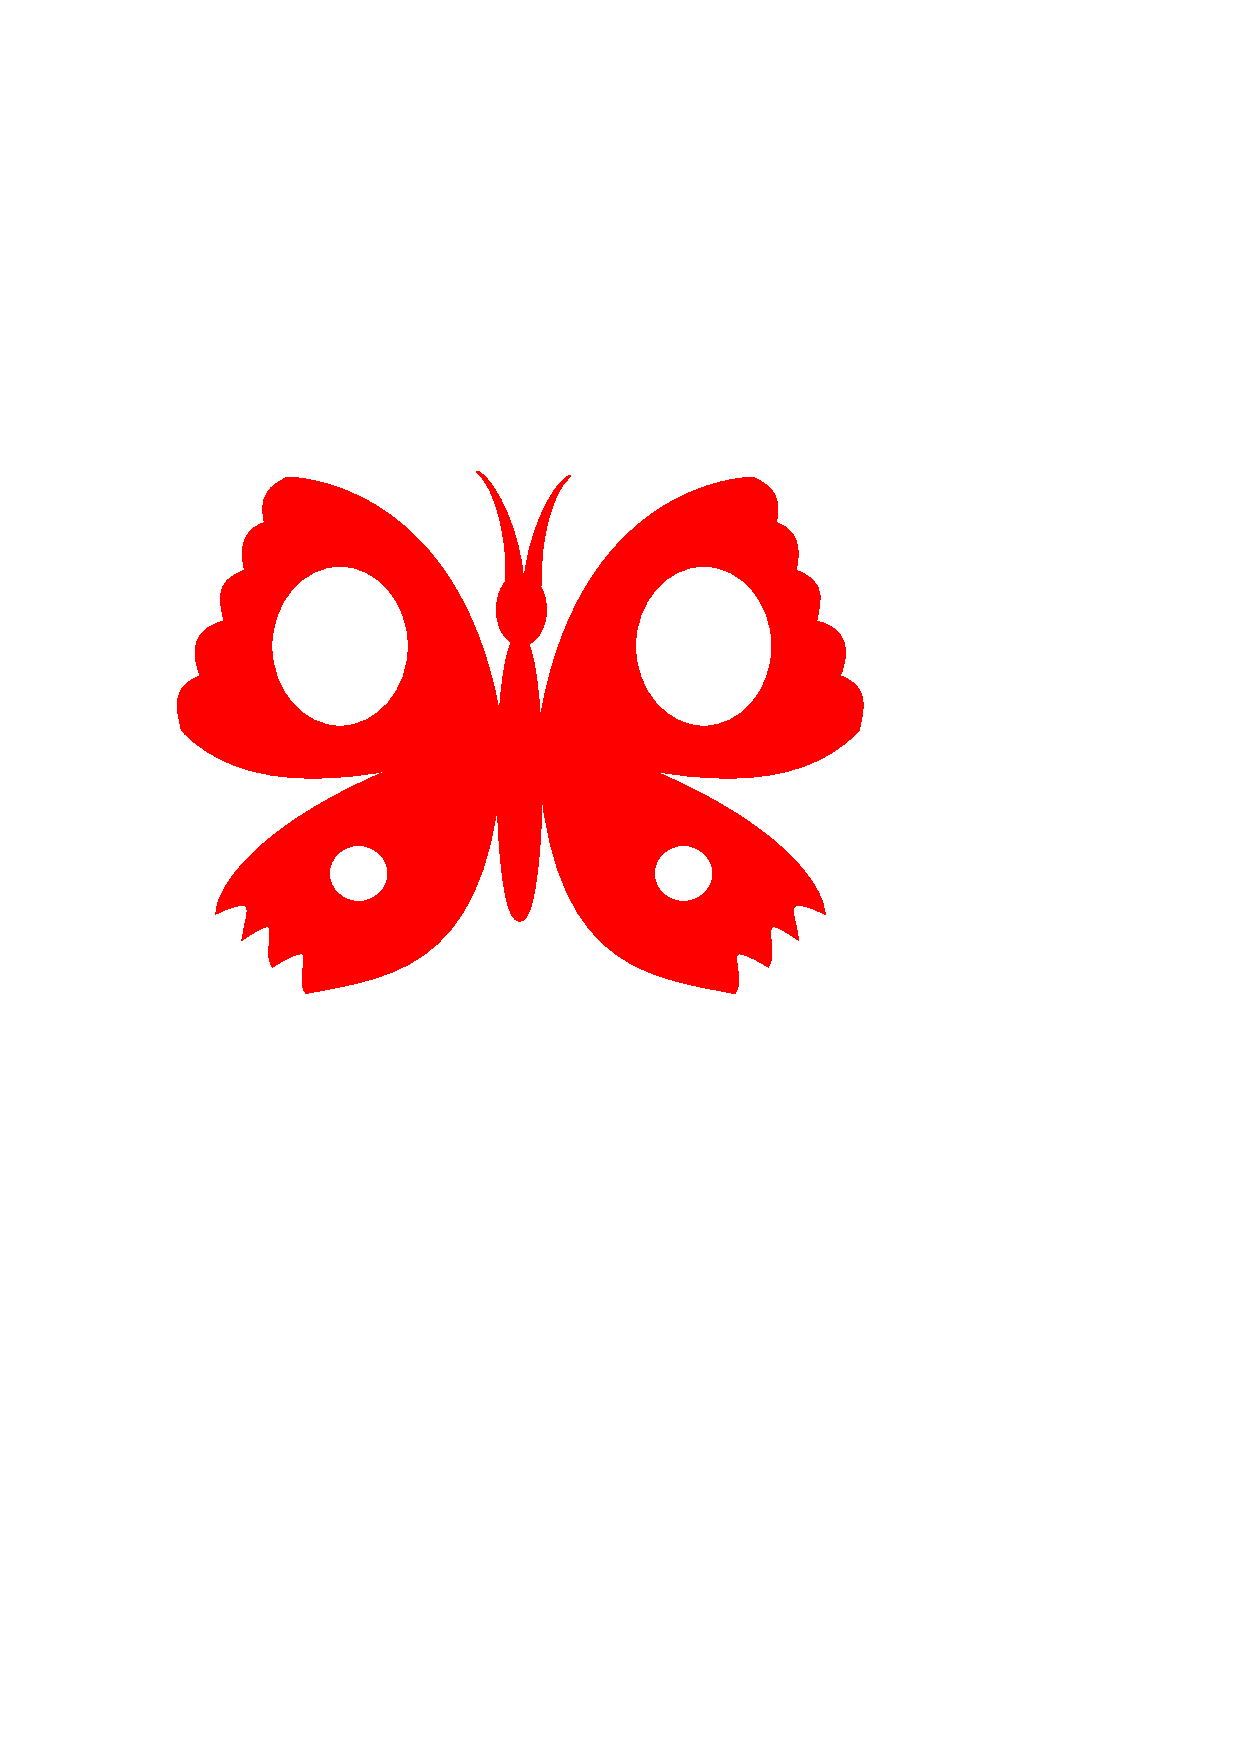
\includegraphics[width=.05\textwidth]{bilder/inkling.pdf}
\end{figure}
Adrìan und Herr Butterblom fangen die Schmetterlinge in der Wohnung ein und bringen sie zurück ins Papiliorama. 

\enquote{Warum haben Sie das getan?} Kommissarin Andermatt spricht die Frage aus, die alle brennend interessiert.

\enquote{Ich wollte, ich, \dots} Frau Studer-Matt kommt ins Stottern. Aber dann holt sie tief Luft und sagt: 

\enquote{Ich wollte das schönste und vollkommenste Kleid nähen, dass je ein Mensch getragen hat. Ich wollte es mit den Flügeln der Schmetterlinge besticken, den schönsten Pailletten der Welt. Das herrliche Blau dieser Schmetterlinge ist einfach unübertroffen. Das ist eine Erfindung, die so genial ist, dass vor mir noch niemand darauf gekommen ist. Ich werde vielleicht verhaftet, aber ich werde in die Modegeschichte eingehen. Das lasse ich mir auch nicht von euch Kleingeistern auch kaputt machen. Was sind schon ein paar Schmetterlinge gegen wahre Schönheit.}

Die Kommissarin schüttelt den Kopf, Carla hat nicht ganz genau verstanden, was Frau Studer-Matt vor hatte und Fenja kann es sich nicht verkneifen zu erklären, dass schon früher Menschen in Süd- und Mittelamerika Kleider mit den Schalen von Käfern bestickt haben. Das ist nicht nur ganz ähnlich, sondern hält auch besser. 

Als die beiden Mädchen zu Hause ankommen, machen Mama und Papa geheimnisvolle Gesichter. 

\enquote{Na, habt ihr heute schön gespielt?} wollen sie wissen. Und noch während Fenja überlegt, ob man auch nicht schön spielen kann, zückt Papa zwei Eintrittskarten hinter dem Rücken hervor.

\enquote{Überraschung: Morgen fahren wir alle zusammen nach Kerzers ins Papiliorama!} Da rufen die beiden Schwestern wie aus einem Mund:

\enquote{Oh nein, bloss nicht! Lieber ins Aquarium ins Dählhölzli.} \hfill {\color{red}\decofourleft}

\vspace{25pt}
\begin{figure}[h]
\centering
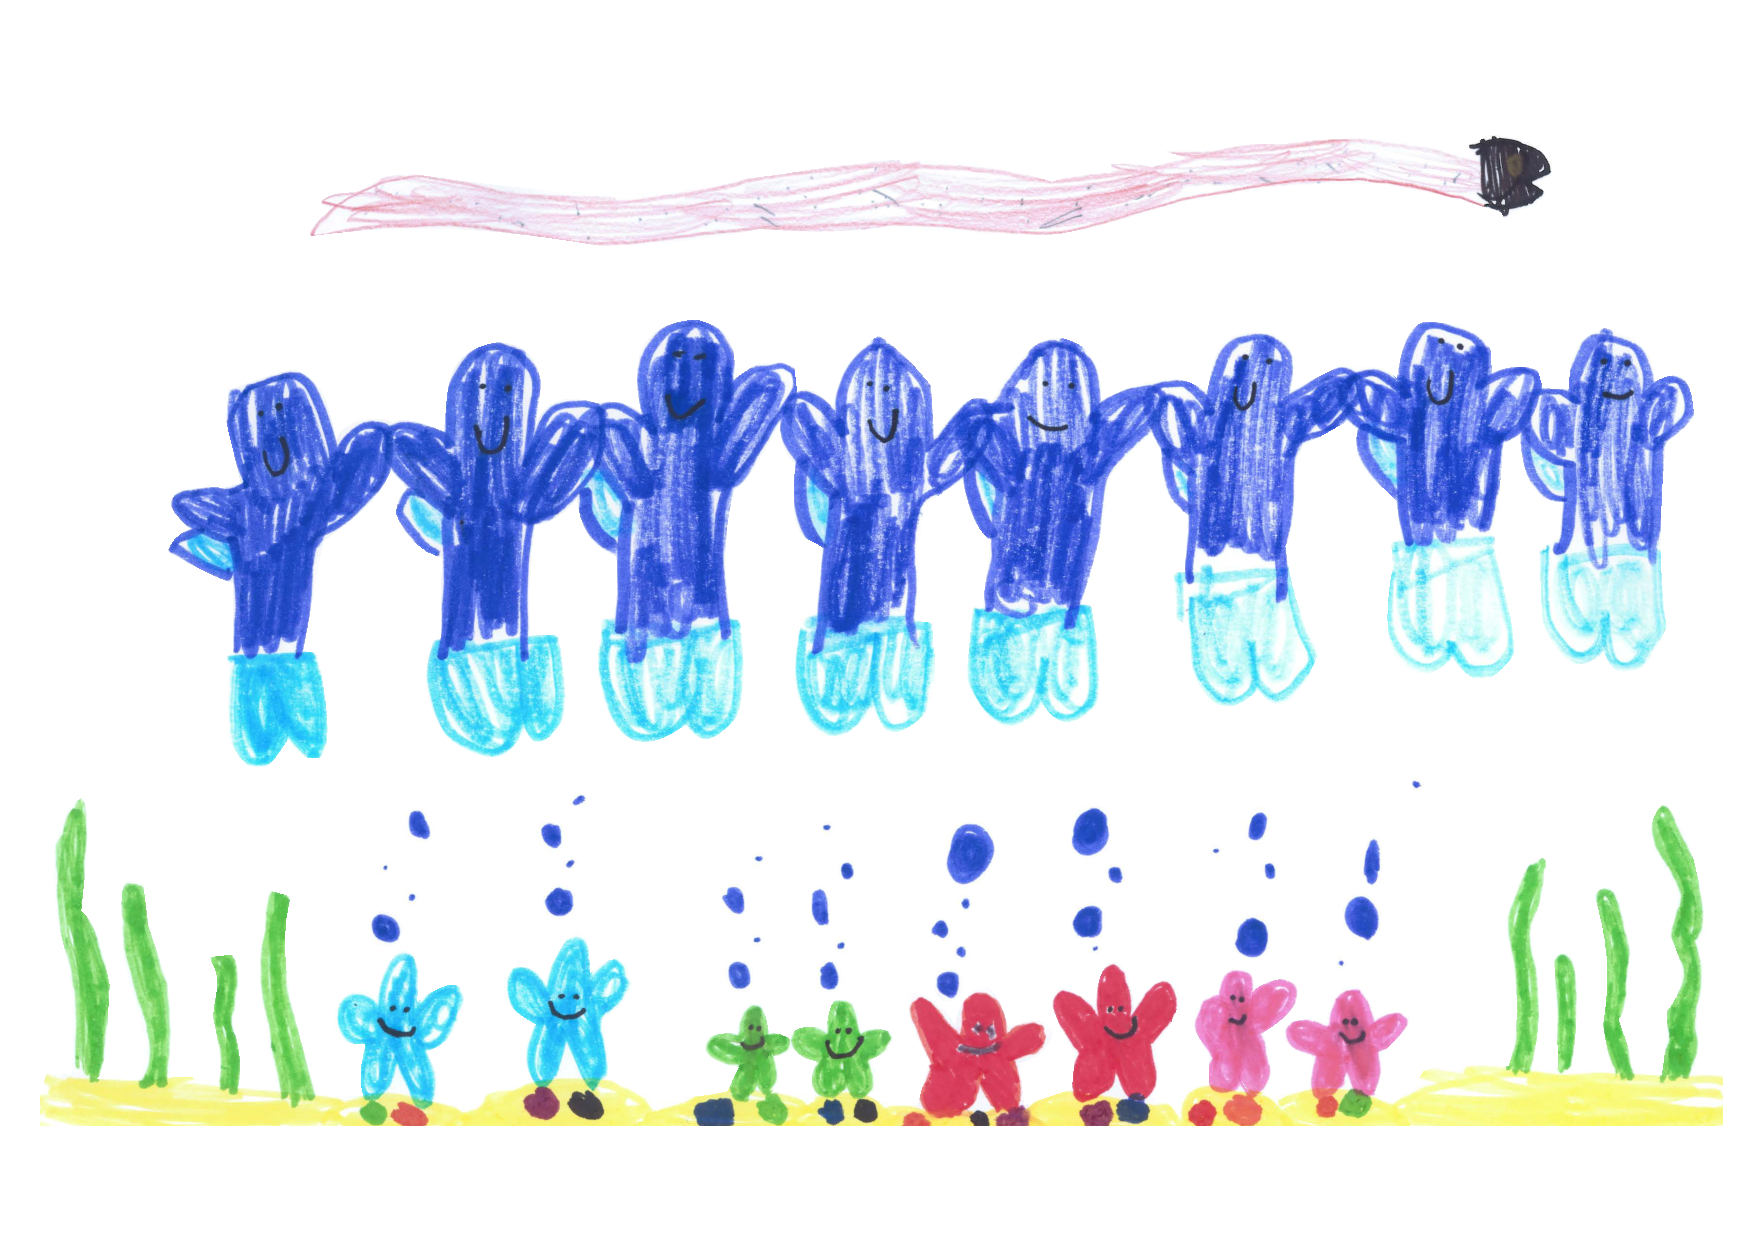
\includegraphics[width=\textwidth]{bilder/kerzers2.pdf}
\end{figure}

